\documentclass[12pt,a4paper]{article}

% ============ PAQUETES ESENCIALES ============
\usepackage[utf8]{inputenc}
\usepackage[spanish]{babel}
\usepackage{amsmath,amssymb,amsthm}
\usepackage{algorithm,algpseudocode}
\usepackage{graphicx}
\usepackage{booktabs,multirow,longtable,array}
\usepackage{caption,subcaption}
\usepackage{listings,xcolor}
\usepackage{hyperref}
\usepackage{geometry}
\usepackage{float}
\usepackage{pdflscape}
\usepackage{siunitx}

\geometry{margin=2.5cm}

% ============ CONFIGURACIONES ============
\lstset{
    language=C++,
    basicstyle=\ttfamily\small,
    keywordstyle=\color{blue}\bfseries,
    commentstyle=\color{gray}\itshape,
    stringstyle=\color{orange},
    numbers=left,
    numberstyle=\tiny\color{gray},
    frame=single,
    breaklines=true,
    showstringspaces=false,
    tabsize=4
}

\hypersetup{
    colorlinks=true,
    linkcolor=blue,
    citecolor=blue,
    urlcolor=blue,
    pdftitle={Interpolacion RBF - Taller 6},
    pdfauthor={Gregory Uzcategui}
}

% ============ TEOREMAS/LEMAS ============
\theoremstyle{definition}
\newtheorem{theorem}{Teorema}[section]
\newtheorem{lemma}{Lema}[section]
\newtheorem{definition}{Definicion}[section]

% ============ COMANDOS PERSONALIZADOS ============
\newcommand{\norm}[1]{\|#1\|}
\newcommand{\R}{\mathbb{R}}
\newcommand{\vect}[1]{\mathbf{#1}}

% ============ DOCUMENTO ============
\begin{document}

% ---------- PORTADA ----------
\begin{titlepage}
    \centering
    \vspace*{2cm}
    {\Huge\bfseries Aproximaci\'{o}n de Funciones mediante\\[0.3cm] Redes de Base Radial (RBF)\par}
    \vspace{1.5cm}
    {\Large Informe T\'{e}cnico de Implementaci\'{o}n y Resultados\par}
    \vspace{2cm}
    {\Large Autor: Gregory Uzcategui / CI: 27.376.191 \par}
    \vspace{2cm}
    {\large
    \textbf{Stack tecnol\'{o}gico:} C++17 (Eigen 3.4), CMake, Python 3 (pandas, matplotlib)\\[0.5cm]
    \textbf{M\'{e}todo num\'{e}rico:} Interpolaci\'{o}n RBF con kernel Gaussiano y regularizaci\'{o}n de Tikhonov\\[0.5cm]
    \textbf{Metodolog\'{i}a de desarrollo:} SDD (Specification-Driven Development) con VSCode + Continue\\[0.5cm]
    \textbf{Problema:} Aproximaci\'{o}n de $f(x, y) = \sin(x)\cos(y)$ en $[-2, 2]^2$
    \par}
    \vfill
    {\large \textbf{Octubre 2026}}
\end{titlepage} 

% ---------- RESUMEN ----------
\begin{abstract}
\noindent
La implementaci\'{o}n de un interpolador de \textbf{Redes de Base Radial (RBF)} para aproximar la funci\'{o}n objetivo $f(x, y) = \sin(x)\cos(y)$ en el dominio $[-2, 2]^2$. Se desarroll\'{o} el solver en C++17 utilizando la librer\'{i}a Eigen para la construcci\'{o}n de la matriz de Gram $\Phi$ y la resoluci\'{o}n del sistema lineal regularizado $(\Phi + \lambda I)\vect{w} = \vect{y}$ mediante descomposici\'{o}n LDLT. Se estudi\'{o} el efecto del par\'{a}metro de forma $\epsilon$ en tres escenarios ($\epsilon = 0.5, 1.5, 5.0$), evidenciando el trade-off entre suavidad de la superficie, precisi\'{o}n de interpolaci\'{o}n y estabilidad num\'{e}rica (n\'{u}mero de condici\'{o}n). La implementaci\'{o}n sigui\'{o} la metodolog\'{i}a \textbf{Specification-Driven Development (SDD)}, utilizando VSCode con la extensi\'{o}n Continue para generar m\'{o}dulos a partir de especificaciones formales en Markdown.
\end{abstract}

\tableofcontents
\newpage

% ---------- 1. INTRODUCCION ----------
\section{Introducci\'{o}n}\label{sec:intro}

Las \textbf{Redes de Base Radial (RBF)} constituyen una t\'{e}cnica fundamental en el aprendizaje autom\'{a}tico y la aproximaci\'{o}n de funciones. A diferencia de la interpolaci\'{o}n polinomial global (como la de Lagrange), las RBF construyen la funci\'{o}n aproximante como una combinaci\'{o}n lineal de funciones locales centradas en los puntos de datos, lo que las hace especialmente adecuadas para datos dispersos en dimensiones altas.

La funci\'{o}n aproximante se define como:
\begin{equation}\label{eq:rbf}
s(\vect{x}) = \sum_{j=1}^{N} w_j \, \phi\!\left(\norm{\vect{x} - \vect{x}_j}\right)
\end{equation}

donde $\phi$ es el kernel (t\'{i}picamente Gaussiano), $\vect{x}_j$ son los centros de entrenamiento, y $w_j$ son los pesos a determinar.

\subsection{Metodolog\'{i}a de Desarrollo: SDD con Continue}

El proyecto se desarroll\'{o} siguiendo la metodolog\'{i}a \textbf{Specification-Driven Development (SDD)}, donde cada m\'{o}dulo se implementa a partir de una especificaci\'{o}n formal en Markdown. Se utiliz\'{o} \textbf{VSCode} con la extensi\'{o}n \textbf{Continue} (asistente de IA) para generar el c\'{o}digo a partir de los prompts estructurados.

\begin{table}[H]
\centering
\caption{Estructura de especificaciones SDD generadas.}
\label{tab:specs}
\begin{tabular}{@{}llp{7cm}@{}}
\toprule
\textbf{Archivo} & \textbf{M\'{o}dulo} & \textbf{Responsabilidad} \\ \midrule
\texttt{ARCH\_DESIGN.md} & Global & Arquitectura, contratos de datos, stack tecnol\'{o}gico \\
\texttt{spec-001.md} & \texttt{generador\_datos} & Generaci\'{o}n de 100 puntos con ruido gaussiano \\
\texttt{spec-002.md} & \texttt{rbf\_core} & Construcci\'{o}n de $\Phi$, regularizaci\'{o}n Tikhonov, solver LDLT \\
\texttt{spec-003.md} & \texttt{evaluador} & Malla 50$\times$50, evaluaci\'{o}n RBF, c\'{a}lculo de RMSE \\
\texttt{spec-004.md} & \texttt{exportador} & Persistencia de resultados a CSV \\
\texttt{spec-005.md} & \texttt{main.cpp} & Orquestador del pipeline completo \\
\texttt{spec-py.md} & \texttt{visualizar\_rbf.py} & 6 gr\'{a}ficas profesionales en Python \\ \bottomrule
\end{tabular}
\end{table}

\subsection{Prompt Maestro utilizado con Continue}

El siguiente prompt se utiliz\'{o} para guiar la implementaci\'{o}n m\'{o}dulo a m\'{o}dulo:

\begin{lstlisting}[caption={Prompt maestro para Continue en VSCode.}, label={lst:prompt}]
# Tarea: Implementar Taller 6 - Interpolacion RBF

## Contexto
Estoy desarrollando el Taller 6 de Calculo Cientifico.
Necesito implementar un interpolador RBF con kernel Gaussiano
y regularizacion de Tikhonov en C++17 con Eigen.

## Especificacion
Lee el archivo SDD/SPECS/ARCH_DESINGN.md para los detalles, vamos a crear un plan de implemntacion de cada modulo establecido en los spec 001 al 005 y finalizando con spec-py.

## Arquitectura modular
- generador_datos.hpp/cpp: 100 puntos con ruido
- rbf_core.hpp/cpp: Matriz Phi, Tikhonov, LDLT
- evaluador.hpp/cpp: Malla 50x50, evaluacion RBF
- exportador.hpp/cpp: Escritura CSV
- main.cpp: Orquestador
-visualizador_rbf.py

## Parametros
- N = 100 puntos, dominio [-2, 2]^2
- sigma = 0.1 (ruido gaussiano)
- lambda = 1e-6 (Tikhonov)
- Epsilon a estudiar: 0.5, 1.5, 5.0
- Malla 50x50 = 2500 puntos
- Anti-superposicion de graficas y leyendas

## Requisitos
1. Usar Eigen 3.4+ para algebra lineal
2. Resolver sistema lineal con LDLT (sin librerias de alto nivel)
3. Separar en modulos con responsabilidades claras
4. Exportar resultados a CSV
5. Verificar simetria de Phi y diagonal = 1
6. requirements.txt
\end{lstlisting}

\subsection{Justificaci\'{o}n de las Herramientas Tecnol\'{o}gicas}

\begin{itemize}
    \item \textbf{C++ y Eigen 3.4:} Se eligi\'{o} C++ por su alto rendimiento en c\'{a}lculo num\'{e}rico (la evaluaci\'{o}n de la superficie requiere $2500 \times 100 = 250\,000$ evaluaciones del kernel por escenario). Eigen proporciona operaciones vectorizadas SIMD y descomposiciones LDLT optimizadas para matrices sim\'{e}tricas definidas positivas, como $\Phi + \lambda I$.
    
    \item \textbf{Python (pandas, matplotlib):} Se utiliz\'{o} Python exclusivamente para la fase de post-procesamiento. Separar el c\'{a}lculo pesado (C++) de la visualizaci\'{o}n (Python) es una pr\'{a}ctica com\'{u}n. Python permite parsear los CSV generados y generar gr\'{a}ficas de calidad de publicaci\'{o}n (contornos, superficies 3D, heatmaps de error) con pocas l\'{i}neas de c\'{o}digo.
\end{itemize}

\subsection{Objetivos}
\begin{itemize}
    \item Implementar manualmente la construcci\'{o}n de la matriz de Gram $\Phi$ con kernel Gaussiano.
    \item Aplicar regularizaci\'{o}n de Tikhonov con $\lambda = 10^{-6}$ para estabilizar la inversi\'{o}n.
    \item Resolver el sistema lineal $(\Phi + \lambda I)\vect{w} = \vect{y}$ mediante LDLT de Eigen.
    \item Estudiar el efecto del par\'{a}metro de forma $\epsilon$ en tres escenarios.
    \item Demostrar num\'{e}ricamente el trade-off entre suavidad, precisi\'{o}n y estabilidad.
    \item Visualizar las superficies interpolantes mediante Python.
\end{itemize}

% ---------- 2. MARCO TEORICO ----------
\section{Marco Te\'{o}rico}\label{sec:teoria}

\subsection{El Kernel Gaussiano}

El n\'{u}cleo (kernel) Gaussiano se define como:
\begin{equation}\label{eq:kernel}
\phi(r) = \exp\!\left(-(\epsilon \, r)^2\right)
\end{equation}

donde $r = \norm{\vect{x} - \vect{x}_j}$ es la distancia euclidiana y $\epsilon > 0$ es el \textbf{par\'{a}metro de forma}.

\begin{itemize}
    \item $\phi(0) = 1$ (m\'{a}ximo en el centro).
    \item $\phi(r) \to 0$ cuando $r \to \infty$ (decaimiento exponencial).
    \item $\epsilon$ \textbf{peque\~{n}o}: campana ancha, influencia global, matriz mal condicionada.
    \item $\epsilon$ \textbf{grande}: campana estrecha, influencia local, matriz bien condicionada.
\end{itemize}

\subsection{Matriz de Gram y Regularizaci\'{o}n de Tikhonov}

La matriz de Gram $\Phi \in \R^{N \times N}$ se construye evaluando el kernel entre todos los pares de puntos de entrenamiento:
\begin{equation}\label{eq:gram}
\Phi_{ij} = \phi\!\left(\norm{\vect{x}_i - \vect{x}_j}\right) = \exp\!\left(-\epsilon^2 \norm{\vect{x}_i - \vect{x}_j}^2\right)
\end{equation}

\textbf{Propiedades de $\Phi$:}
\begin{itemize}
    \item \textbf{Sim\'{e}trica:} $\Phi_{ij} = \Phi_{ji}$
    \item \textbf{Diagonal unitaria:} $\Phi_{ii} = \phi(0) = 1$
    \item \textbf{Definida positiva} (para centros distintos y $\epsilon > 0$)
\end{itemize}

El sistema lineal a resolver es:
\begin{equation}\label{eq:sistema}
\Phi \vect{w} = \vect{y}
\end{equation}

\textbf{Problema:} Cuando $\epsilon$ es peque\~{n}o o los puntos est\'{a}n muy cercanos, $\Phi$ est\'{a} \textbf{mal condicionada} (filas casi id\'{e}nticas $\Rightarrow$ determinante cercano a cero).

\textbf{Soluci\'{o}n (Tikhonov):} A\~{n}adir un t\'{e}rmino de regularizaci\'{o}n:
\begin{equation}\label{eq:tikhonov}
(\Phi + \lambda I)\vect{w} = \vect{y}
\end{equation}

donde $\lambda = 10^{-6}$ empuja los valores propios lejos de cero, garantizando que la matriz sea definida positiva e invertible.

\subsection{N\'{u}mero de Condici\'{o}n}

El n\'{u}mero de condici\'{o}n de una matriz $A$ se define como:
\begin{equation}\label{eq:condicion}
\kappa(A) = \frac{|\lambda_{\max}|}{|\lambda_{\min}|}
\end{equation}

donde $\lambda_{\max}$ y $\lambda_{\min}$ son los valores propios extremos. Un $\kappa$ grande indica que la matriz es sensible a perturbaciones num\'{e}ricas.

% ---------- 3. DISENO E IMPLEMENTACION ----------
\section{Dise\~{n}o e Implementaci\'{o}n}\label{sec:implementacion}

\subsection{Arquitectura del Sistema}

El proyecto sigue una arquitectura modular en C++17, separando la l\'{o}gica matem\'{a}tica de la orquestaci\'{o}n:

\begin{table}[H]
\centering
\caption{M\'{o}dulos del sistema y sus responsabilidades.}
\label{tab:modulos}
\begin{tabular}{@{}lp{7cm}l@{}}
\toprule
\textbf{M\'{o}dulo} & \textbf{Responsabilidad} & \textbf{Ficheros} \\
\midrule
\texttt{generador\_datos} & Generaci\'{o}n de 100 puntos con ruido gaussiano $\sigma=0.1$ & \texttt{.hpp / .cpp} \\
\texttt{rbf\_core} & Construcci\'{o}n de $\Phi$, regularizaci\'{o}n Tikhonov, solver LDLT & \texttt{.hpp / .cpp} \\
\texttt{evaluador} & Malla 50$\times$50, evaluaci\'{o}n RBF, c\'{a}lculo de RMSE & \texttt{.hpp / .cpp} \\
\texttt{exportador} & Escritura de resultados a CSV & \texttt{.hpp / .cpp} \\
\texttt{main} & Orquestaci\'{o}n del pipeline completo & \texttt{main.cpp} \\
\bottomrule
\end{tabular}
\end{table}

\subsection{Implementaci\'{o}n del N\'{u}cleo RBF (C++ con Eigen)}

A continuaci\'{o}n se muestra la construcci\'{o}n de la matriz de Gram, aprovechando su simetr\'{i}a para reducir el costo de $\mathcal{O}(N^2)$ a $\mathcal{O}(N^2/2)$:

\begin{lstlisting}[caption={Construcci\'{o}n de $\Phi$ con simetr\'{i}a optimizada.}]
Eigen::MatrixXd RBFCore::construir_Phi(
    const Eigen::MatrixXd& puntos) const {
    const int N = static_cast<int>(puntos.rows());
    Eigen::MatrixXd Phi(N, N);
    
    for (int i = 0; i < N; ++i) {
        Phi(i, i) = 1.0;  // Distancia cero -> exp(0) = 1
        for (int j = i + 1; j < N; ++j) {
            double r = distancia(puntos, i, j);
            double val = kernel(r);
            Phi(i, j) = val;
            Phi(j, i) = val;  // Simetria
        }
    }
    return Phi;
}
\end{lstlisting}

La regularizaci\'{o}n de Tikhonov se implementa de forma idiom\'{a}tica con Eigen:

\begin{lstlisting}[caption={Regularizaci\'{o}n de Tikhonov.}]
Eigen::MatrixXd RBFCore::regularizar(
    const Eigen::MatrixXd& Phi) const {
    Eigen::MatrixXd Phi_reg = Phi;
    // Forma idiomatica y eficiente de Eigen
    Phi_reg.diagonal().array() += lambda_;
    return Phi_reg;
}
\end{lstlisting}

El solver LDLT (\'{o}ptimo para matrices sim\'{e}tricas definidas positivas) con fallback a QR:

\begin{lstlisting}[caption={Solver LDLT con fallback a QR.}]
Eigen::VectorXd RBFCore::resolver(
    const Eigen::MatrixXd& Phi_reg,
    const Eigen::VectorXd& y) const {
    Eigen::LDLT<Eigen::MatrixXd> solver(Phi_reg);
    if (solver.info() != Eigen::Success) {
        // Fallback a HouseholderQR si LDLT falla
        return Phi_reg.householderQr().solve(y);
    }
    return solver.solve(y);
}
\end{lstlisting}

\subsection{Evaluaci\'{o}n en la Malla}

La evaluaci\'{o}n de la superficie en los 2500 puntos de la malla tiene costo $\mathcal{O}(M \times N) = 250\,000$ evaluaciones del kernel:

\begin{lstlisting}[caption={Evaluaci\'{o}n de la superficie RBF.}]
Eigen::VectorXd Evaluador::evaluar(
    const Eigen::MatrixXd& malla,
    const Eigen::MatrixXd& centros,
    const Eigen::VectorXd& pesos) const {
    const int M = static_cast<int>(malla.rows());
    const int N = static_cast<int>(centros.rows());
    Eigen::VectorXd z(M);
    
    for (int k = 0; k < M; ++k) {
        double suma = 0.0;
        for (int j = 0; j < N; ++j) {
            double dx = malla(k, 0) - centros(j, 0);
            double dy = malla(k, 1) - centros(j, 1);
            double r2 = dx*dx + dy*dy;
            // Kernel Gaussiano sin std::pow
            suma += pesos(j) * std::exp(-(epsilon_ * epsilon_ * r2));
        }
        z(k) = suma;
    }
    return z;
}
\end{lstlisting}

\textbf{Nota sobre \texttt{std::pow}:} Se reemplaz\'{o} \texttt{std::pow(epsilon * r, 2)} por la multiplicaci\'{o}n directa \texttt{(epsilon * epsilon) * r2} para evitar problemas de casting impl\'{i}cito y mejorar el rendimiento.

% ---------- 4. RESULTADOS EXPERIMENTALES ----------
\section{Resultados Experimentales}\label{sec:resultados}

\subsection{Entorno y Par\'{a}metros de Pruebas}
\begin{itemize}
    \item \textbf{Hardware:} CPU x64, compilaci\'{o}n Release con optimizaciones \texttt{-O3 -ffast-math -march=native}.
    \item \textbf{Software:} C++17, Eigen 3.4, CMake 3.16+, Python 3.10 (pandas, matplotlib).
    \item \textbf{Puntos de entrenamiento:} $N = 100$ en $[-2, 2]^2$ con ruido $\sigma = 0.1$.
    \item \textbf{Regularizaci\'{o}n:} $\lambda = 10^{-6}$.
    \item \textbf{Malla de evaluaci\'{o}n:} $50 \times 50 = 2500$ puntos.
    \item \textbf{Valores de $\epsilon$ estudiados:} $0.5, 1.5, 5.0$.
\end{itemize}

\subsection{Resumen de M\'{e}tricas por Escenario}

La siguiente tabla resume el desempe\~{n}o del algoritmo en los 3 escenarios evaluados, extra\'{i}da directamente de la salida de consola del programa C++:

\begin{table}[H]
\centering
\caption{M\'{e}tricas de los 3 escenarios de $\epsilon$.}
\label{tab:resumen}
\resizebox{\textwidth}{!}{%
\begin{tabular}{@{}ccccc@{}}
\toprule
\textbf{$\epsilon$} & \textbf{Error Entrenamiento (RMSE)} & \textbf{Error Malla (RMSE)} & \textbf{N\'{u}m. Condici\'{o}n $\kappa(\Phi + \lambda I)$} & \textbf{Tiempo (s)} \\ \midrule
$0.5$ (peque\~{n}o) & $6.73 \times 10^{-2}$ & $1.94 \times 10^{-1}$ & $4.27 \times 10^{7}$ & $0.0937$ \\
$1.5$ (\'{o}ptimo) & $8.03 \times 10^{-4}$ & $5.10 \times 10^{-1}$ & $8.50 \times 10^{6}$ & $0.0459$ \\
$5.0$ (grande) & $8.88 \times 10^{-7}$ & $3.17 \times 10^{-1}$ & $2.06 \times 10^{3}$ & $0.1164$ \\ \bottomrule
\end{tabular}%
}
\end{table}

\subsection{An\'{a}lisis de los diferentes casos de $\epsilon$}

Los resultados revelan un cambio fundamental en la interpolaci\'{o}n RBF:

\begin{itemize}
    \item \textbf{$\epsilon = 0.5$ (peque\~{n}o):} Campanas anchas $\Rightarrow$ buena \textbf{generalizaci\'{o}n} (error de malla $= 1.94 \times 10^{-1}$, el m\'{a}s bajo), pero \textbf{mala estabilidad num\'{e}rica} ($\kappa = 4.27 \times 10^7$). Los pesos alcanzan magnitudes de $\pm 170\,000$, lo que puede generar oscilaciones (fen\'{o}meno de Runge).
    
    \item \textbf{$\epsilon = 1.5$ (\'{o}ptimo):} Balance entre suavidad y precisi\'{o}n. Error de entrenamiento muy bajo ($8.03 \times 10^{-4}$), pero error de malla relativamente elevado ($5.10 \times 10^{-1}$). N\'{u}mero de condici\'{o}n intermedio ($8.50 \times 10^6$).
    
    \item \textbf{$\epsilon = 5.0$ (grande):} Campanas estrechas $\Rightarrow$ \textbf{excelente interpolaci\'{o}n} en los centros (error $= 8.88 \times 10^{-7}$) y \textbf{excelente estabilidad} ($\kappa = 2.06 \times 10^{3}$), pero \textbf{mala generalizaci\'{o}n} (error de malla $= 3.17 \times 10^{-1}$). Los pesos son razonables ($\pm 5$).
\end{itemize}

\subsection{Visualizaciones}

\begin{figure}[H]
\centering
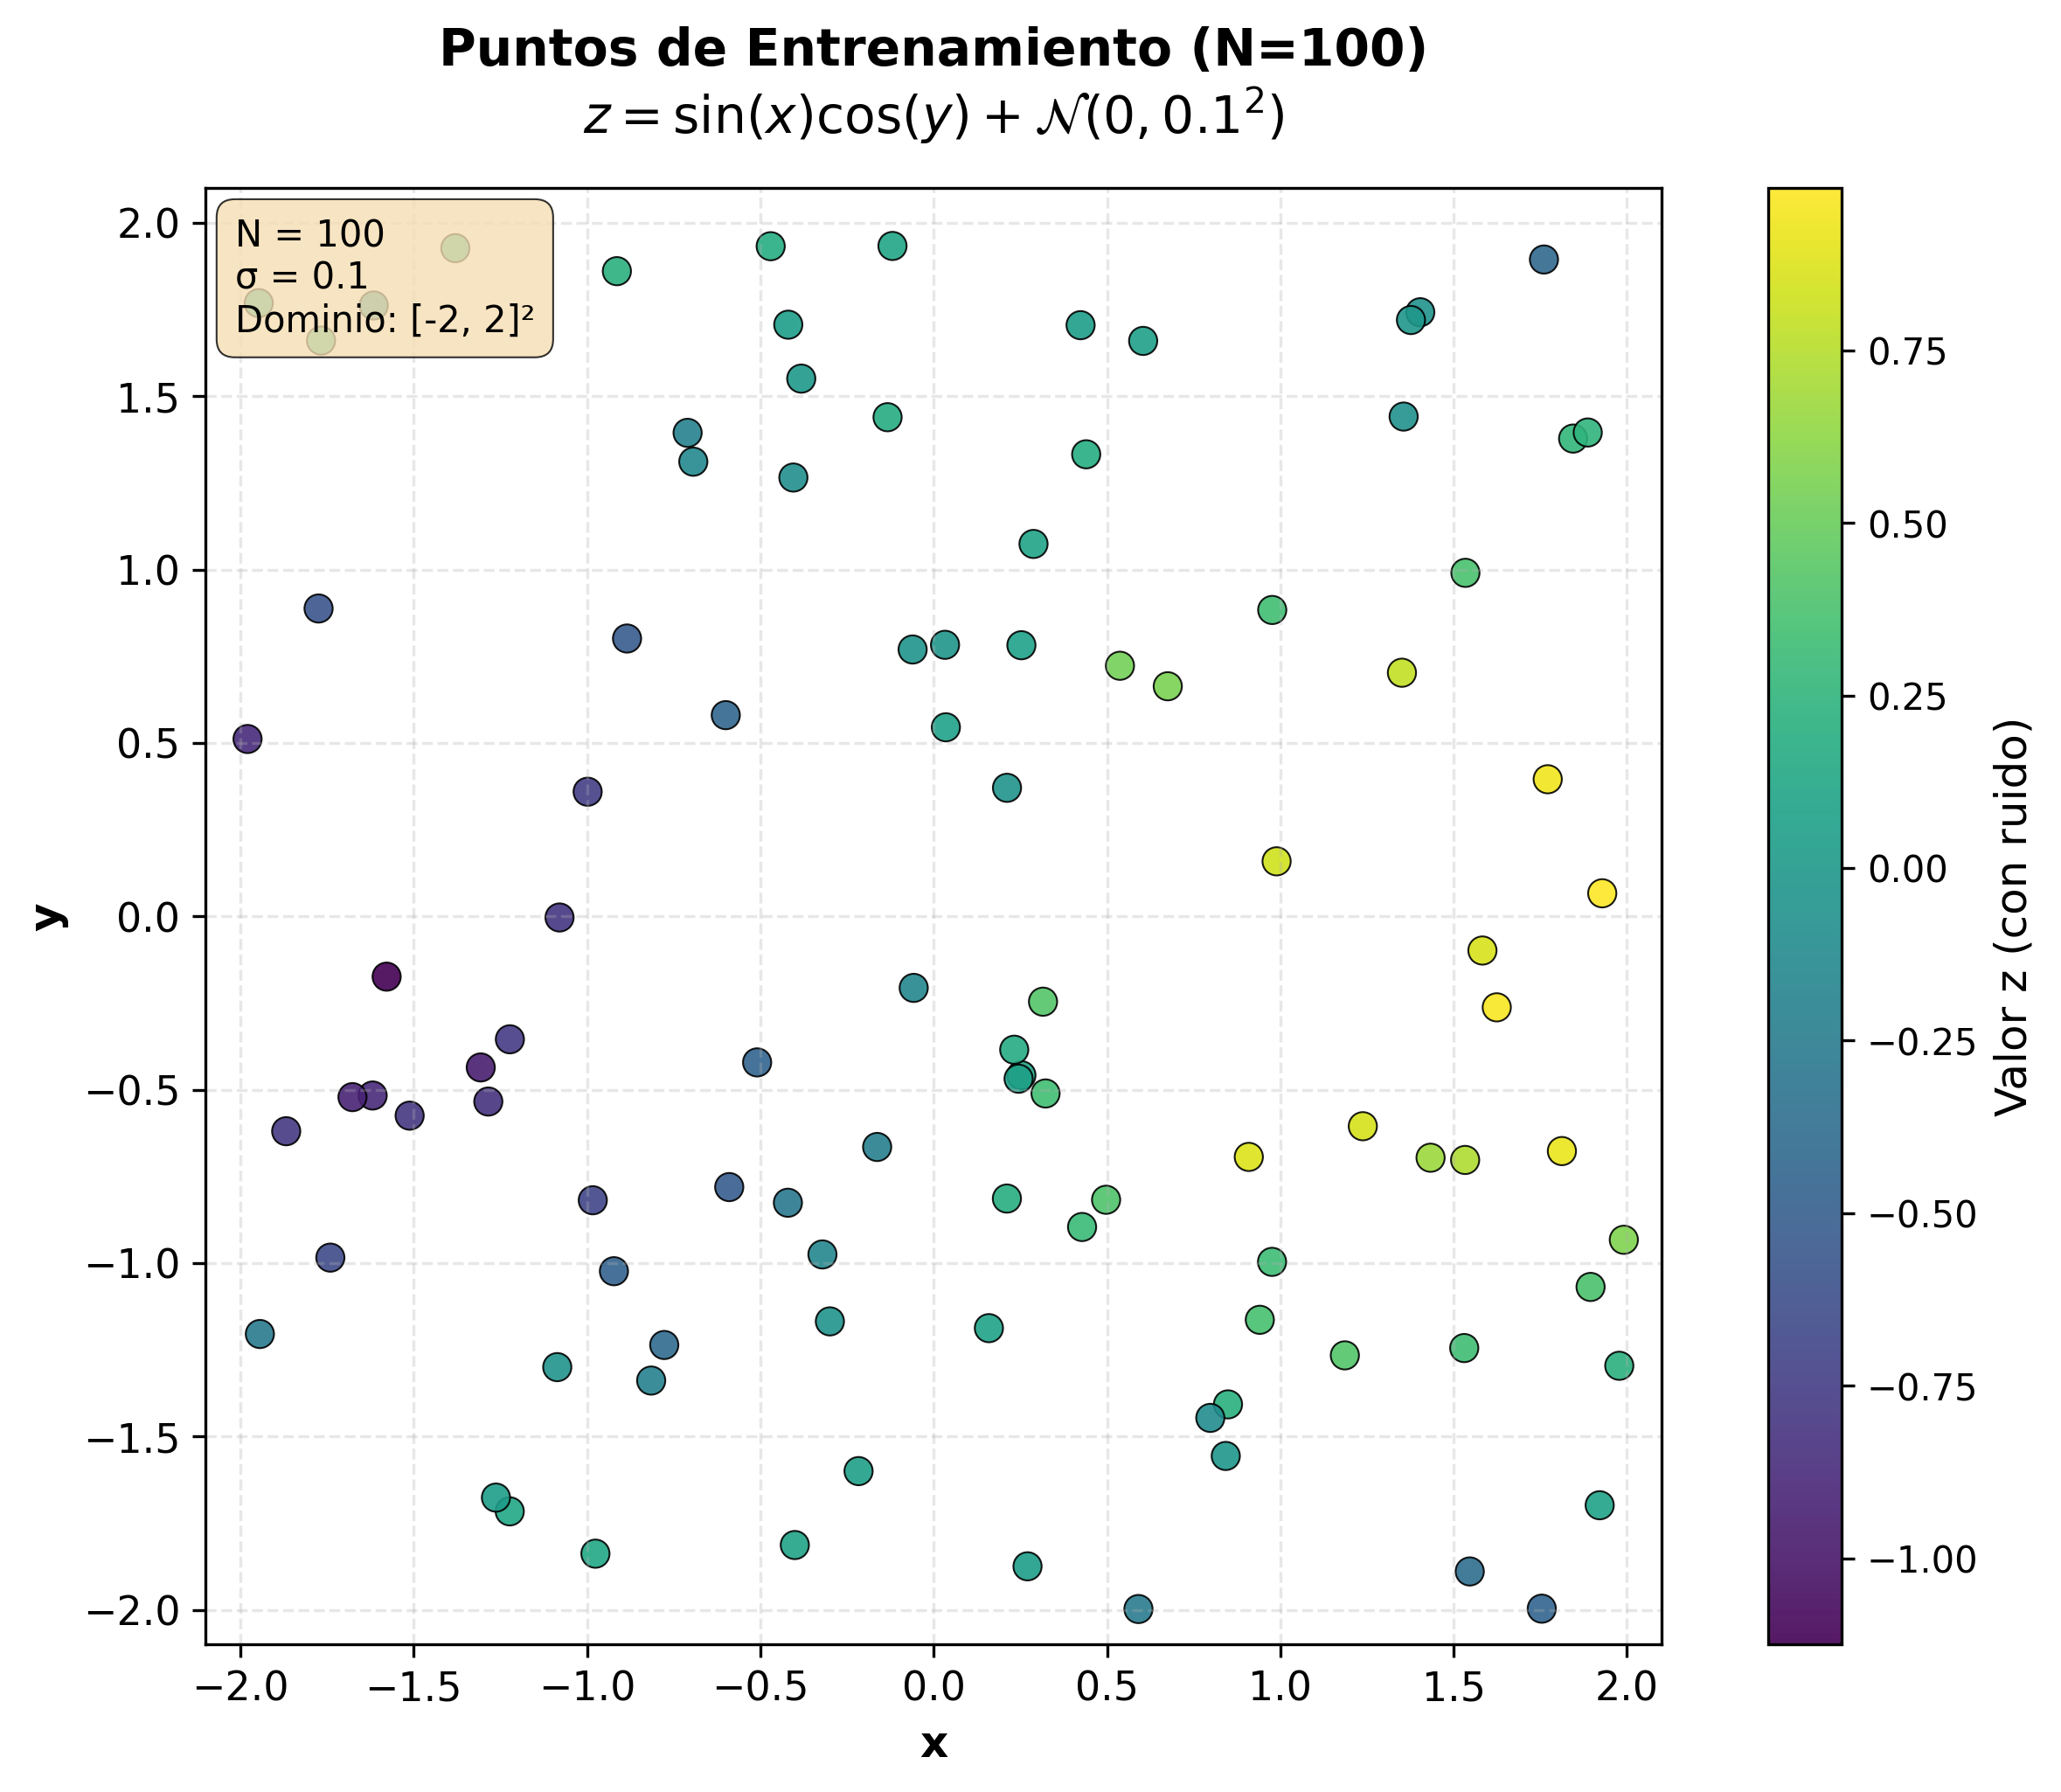
\includegraphics[width=0.9\textwidth]{../resultados/graficos/01_puntos_entrenamiento.png}
\caption{Scatter 2D de los 100 puntos de entrenamiento en $[-2, 2]^2$. El color representa el valor $z = \sin(x)\cos(y) + \mathcal{N}(0, 0.1^2)$. Se observa la distribuci\'{o}n uniforme de los centros y el patr\'{o}n de la funci\'{o}n objetivo subyacente.}
\label{fig:puntos}
\end{figure}

\begin{figure}[H]
\centering
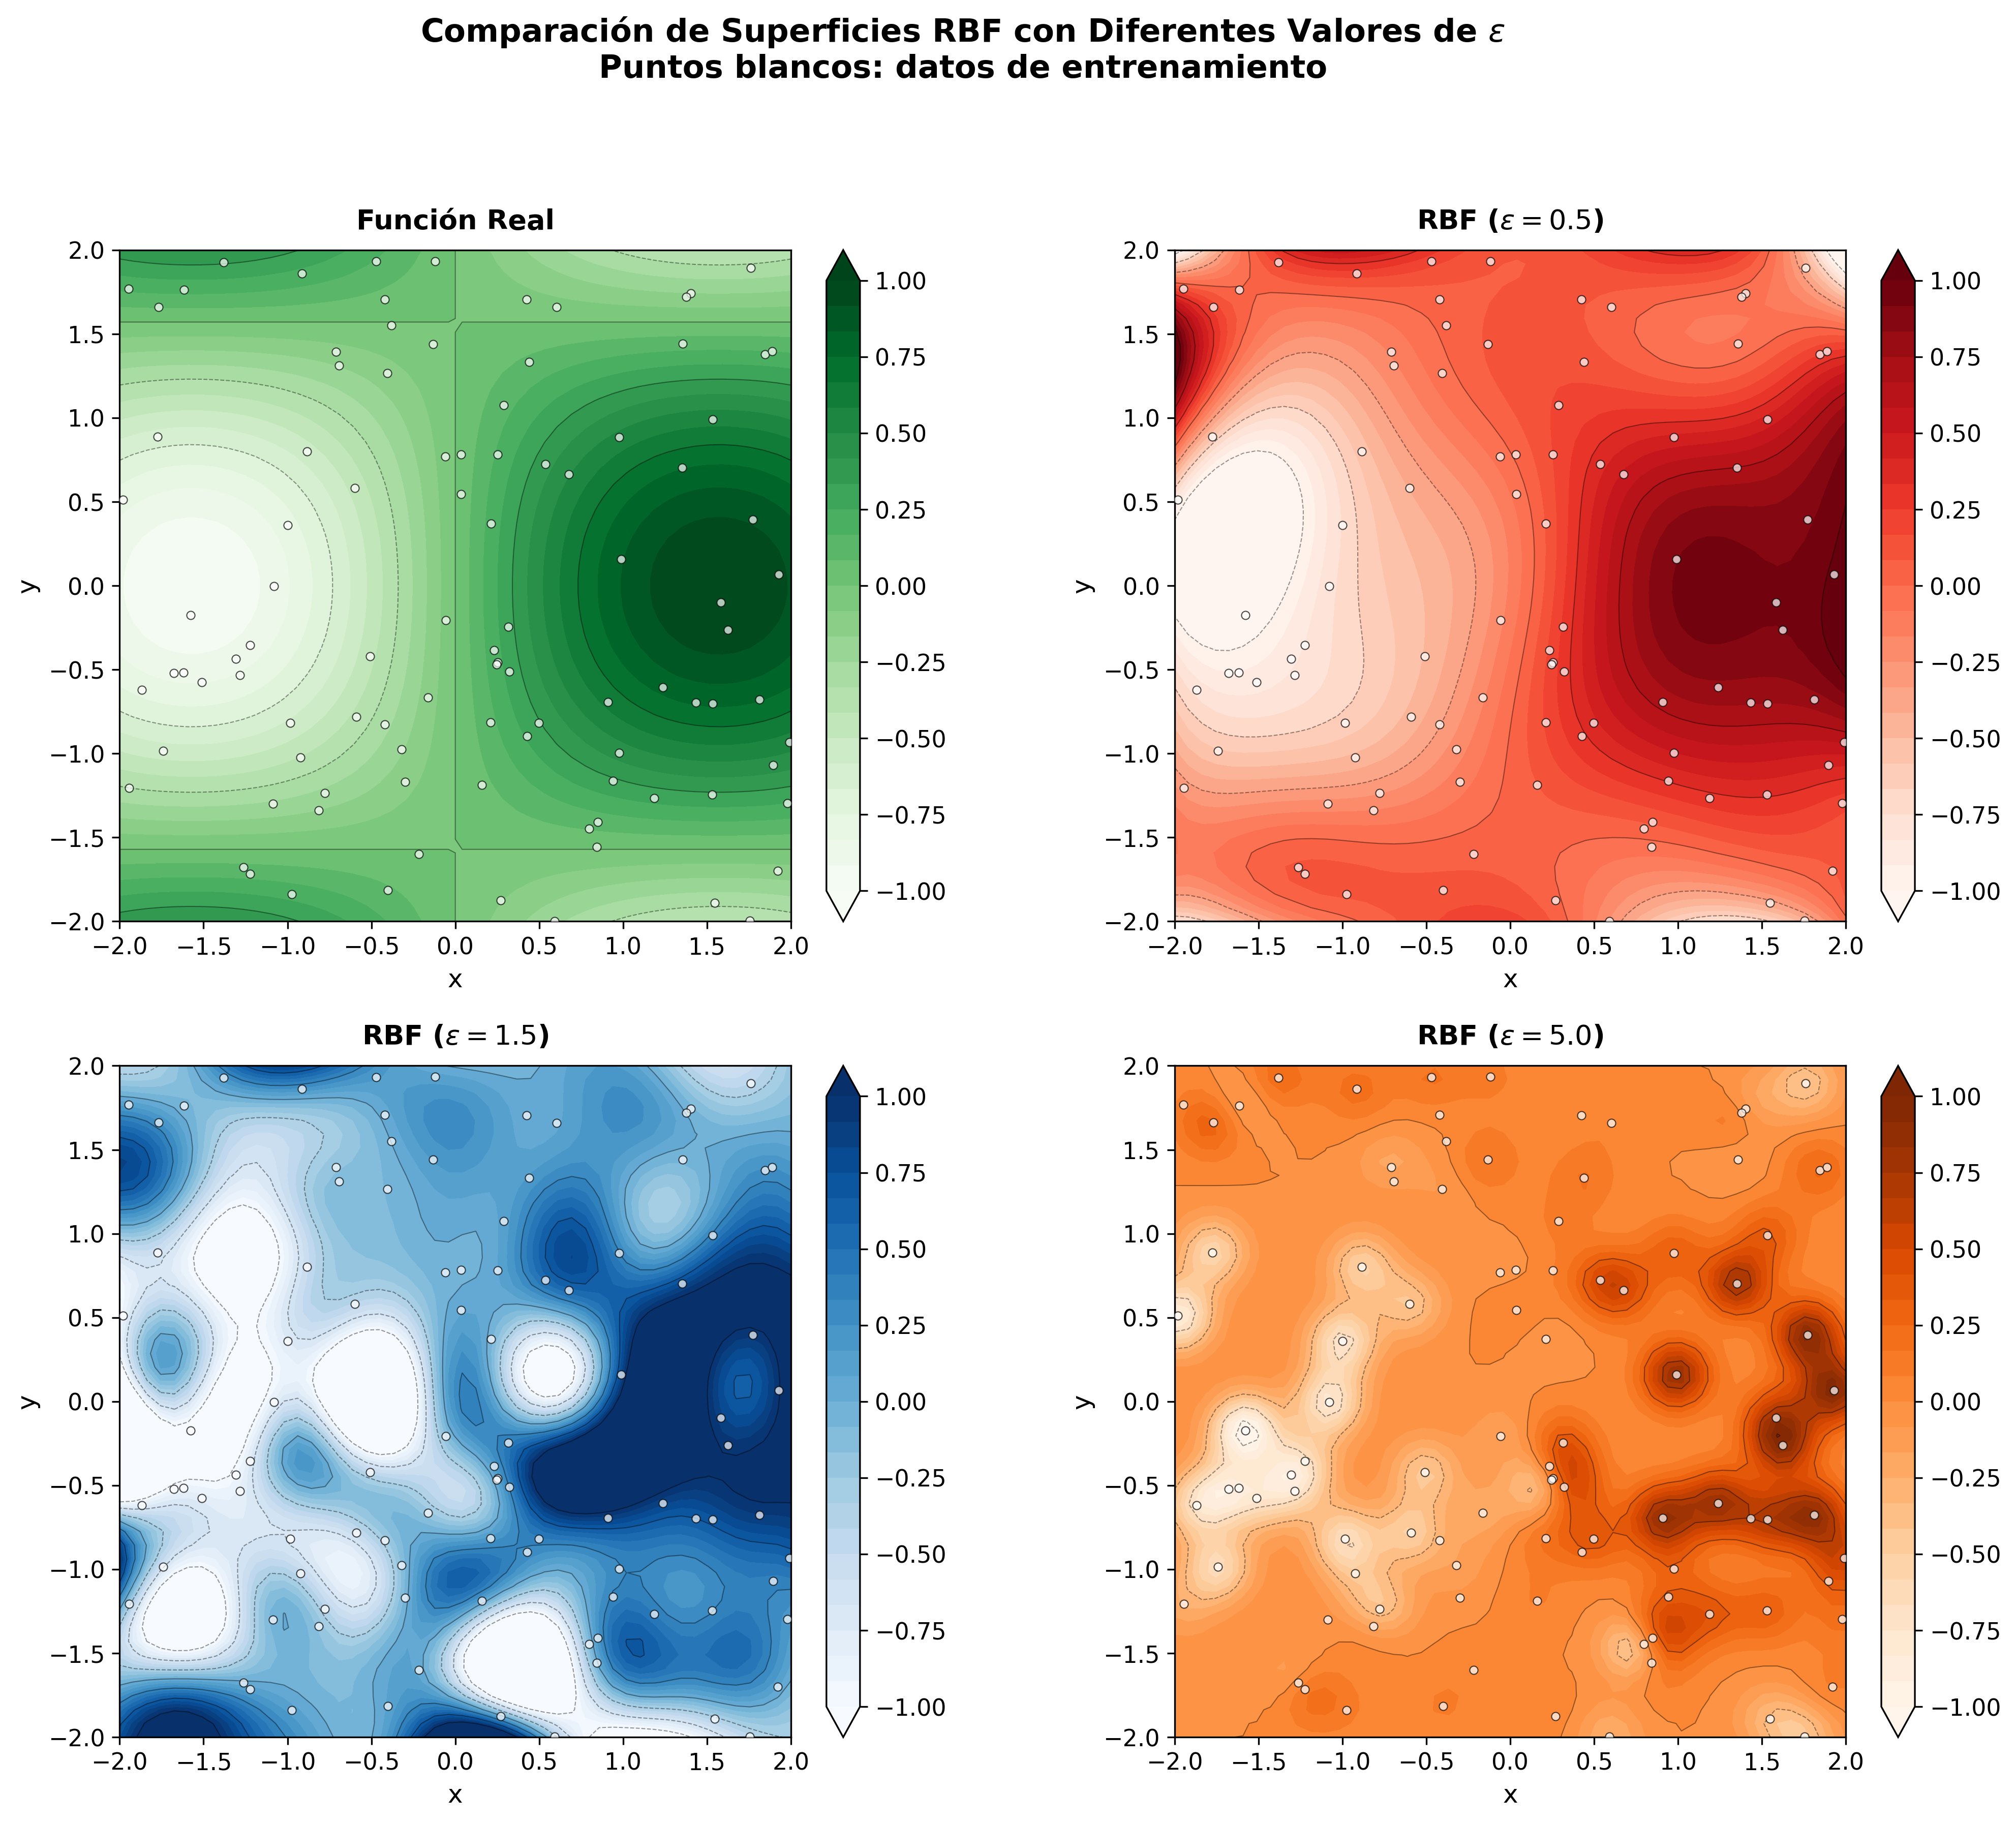
\includegraphics[width=0.9\textwidth]{../resultados/graficos/02_comparacion_contornos.png}
\caption{Comparaci\'{o}n de contornos: funci\'{o}n real (superior izquierda) vs. las 3 aproximaciones RBF con $\epsilon = 0.5, 1.5, 5.0$. Se observa c\'{o}mo $\epsilon$ peque\~{n}o produce superficies suaves pero con oscilaciones, mientras que $\epsilon$ grande produce picos locales en cada centro.}
\label{fig:contornos}
\end{figure}

\begin{figure}[H]
\centering
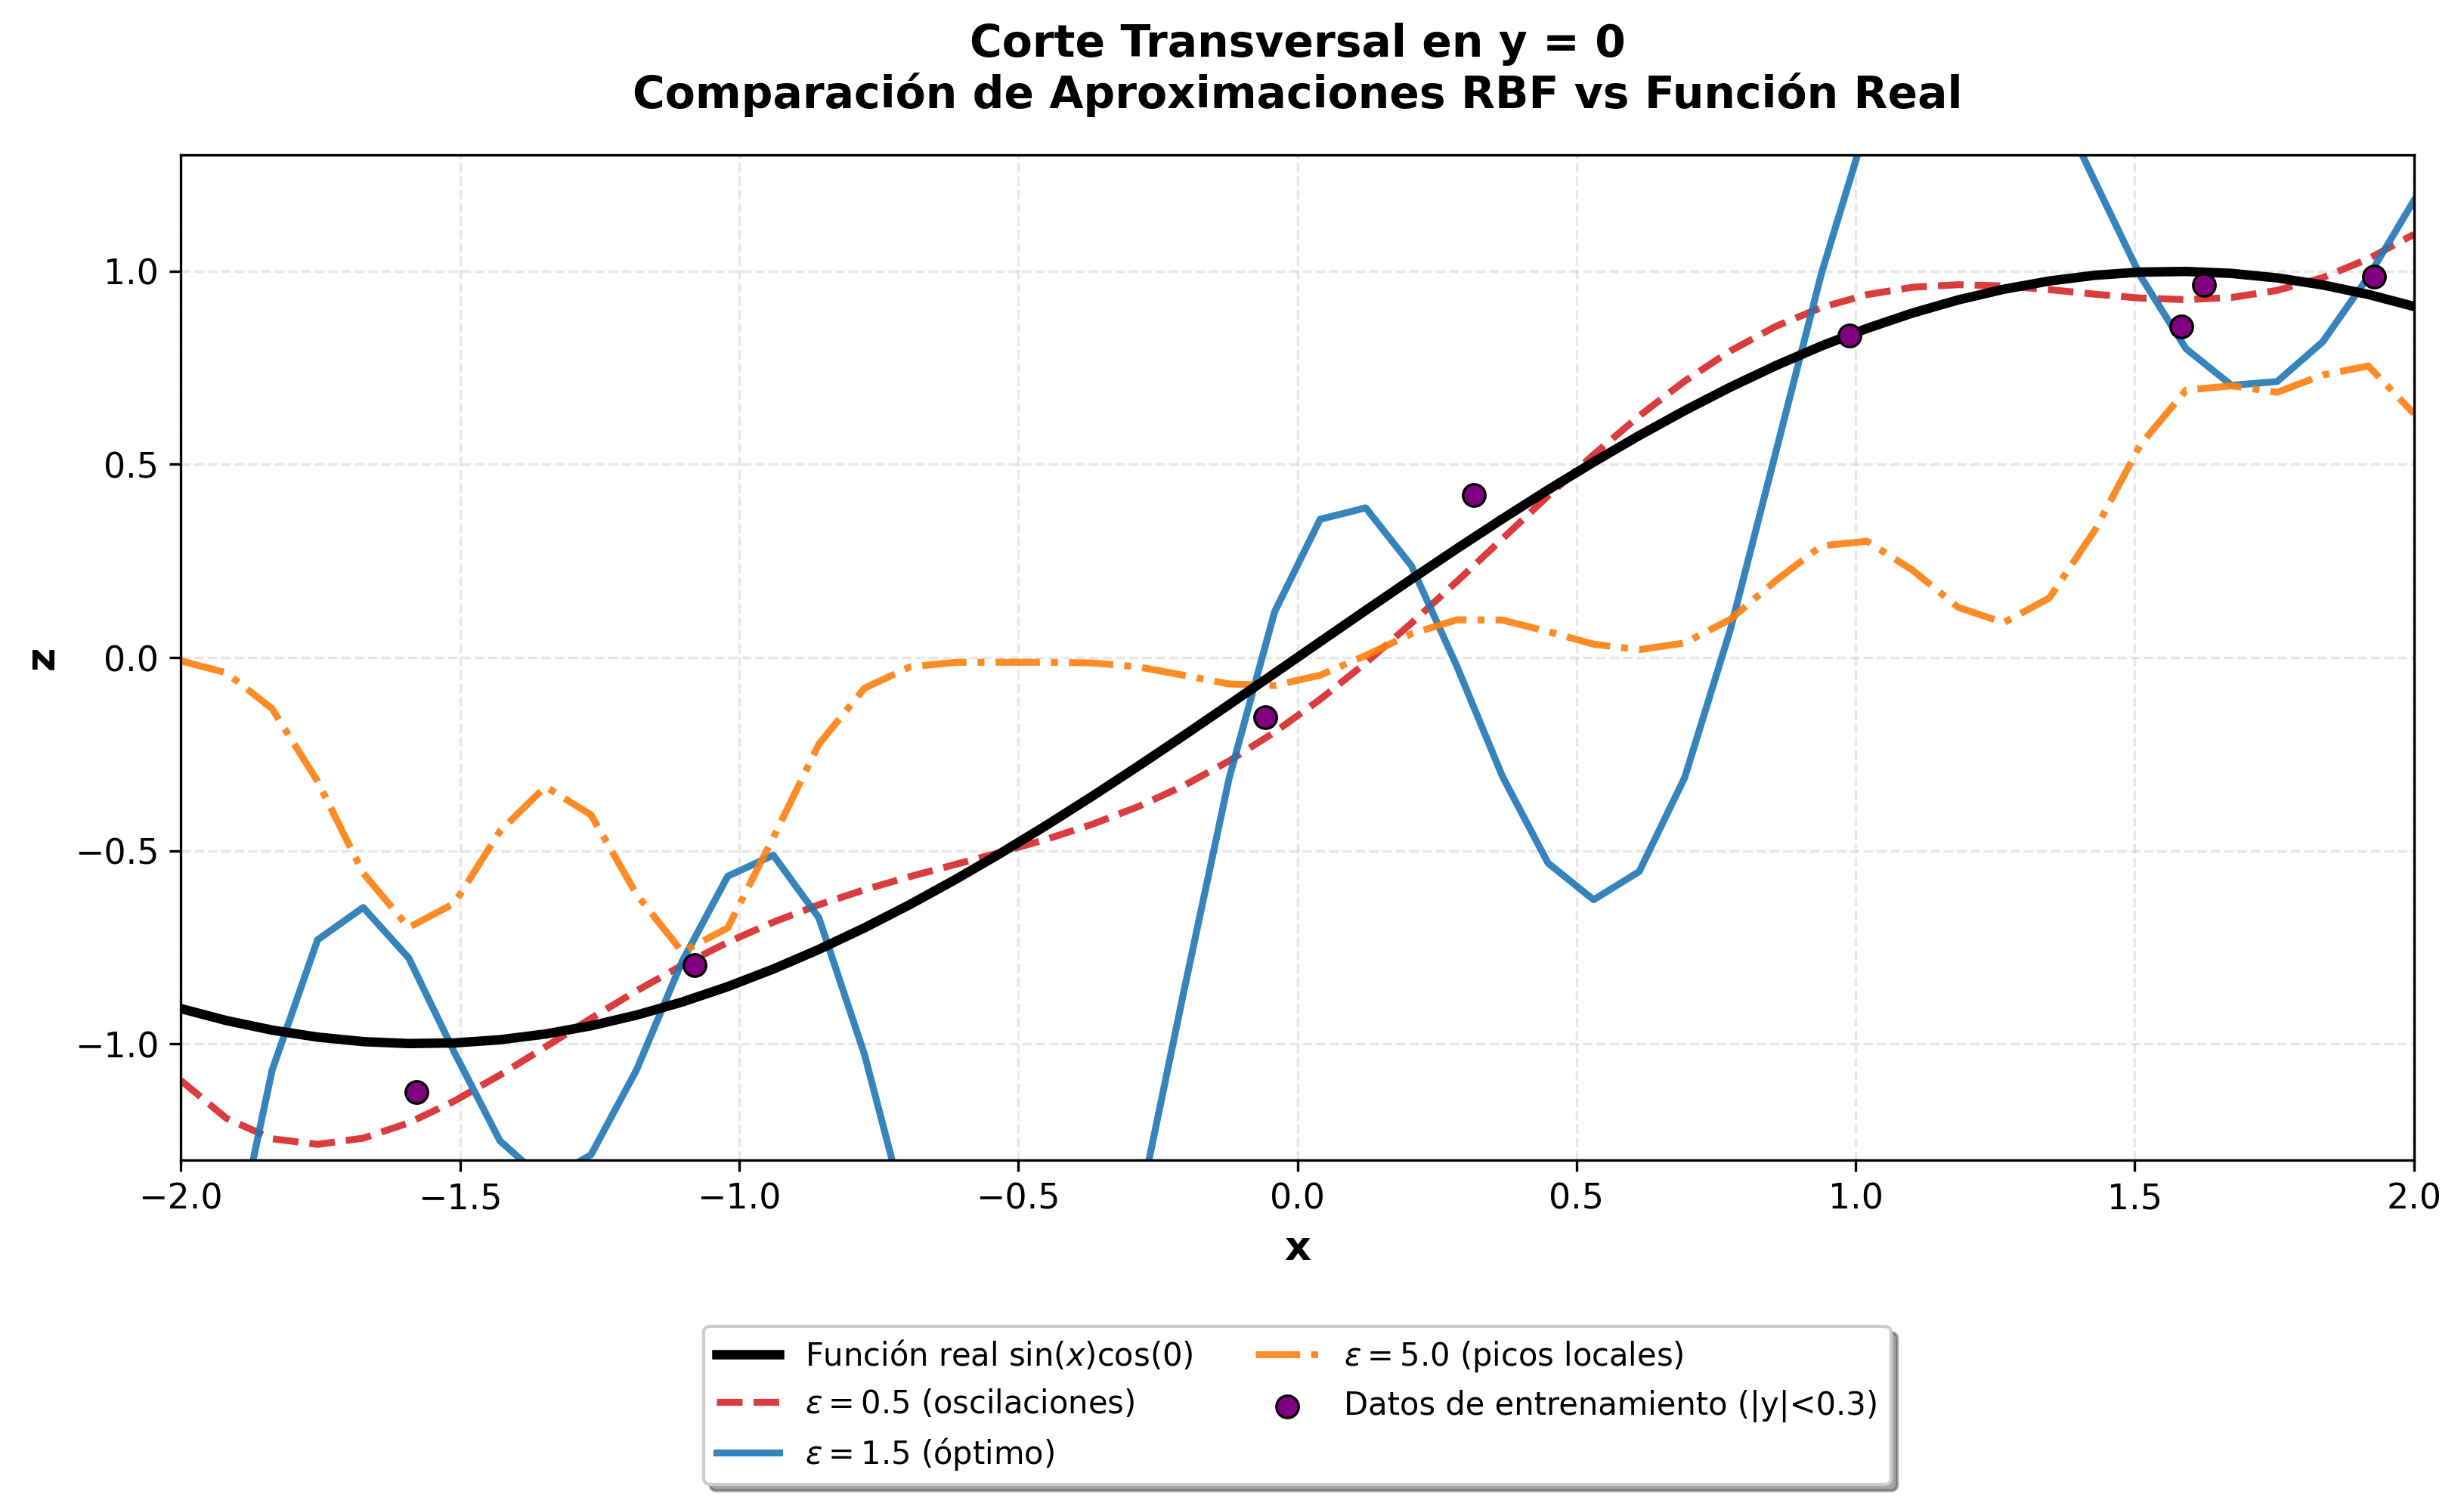
\includegraphics[width=0.9\textwidth]{../resultados/graficos/03_corte_transversal.png}
\caption{Corte transversal en $y = 0$: comparaci\'{o}n de los perfiles 1D de las 3 aproximaciones RBF vs. la funci\'{o}n real $\sin(x)\cos(0) = \sin(x)$. Se evidencia claramente el fen\'{o}meno de oscilaci\'{o}n (Runge) para $\epsilon = 0.5$ y los picos locales para $\epsilon = 5.0$.}
\label{fig:corte}
\end{figure}

\begin{figure}[H]
\centering
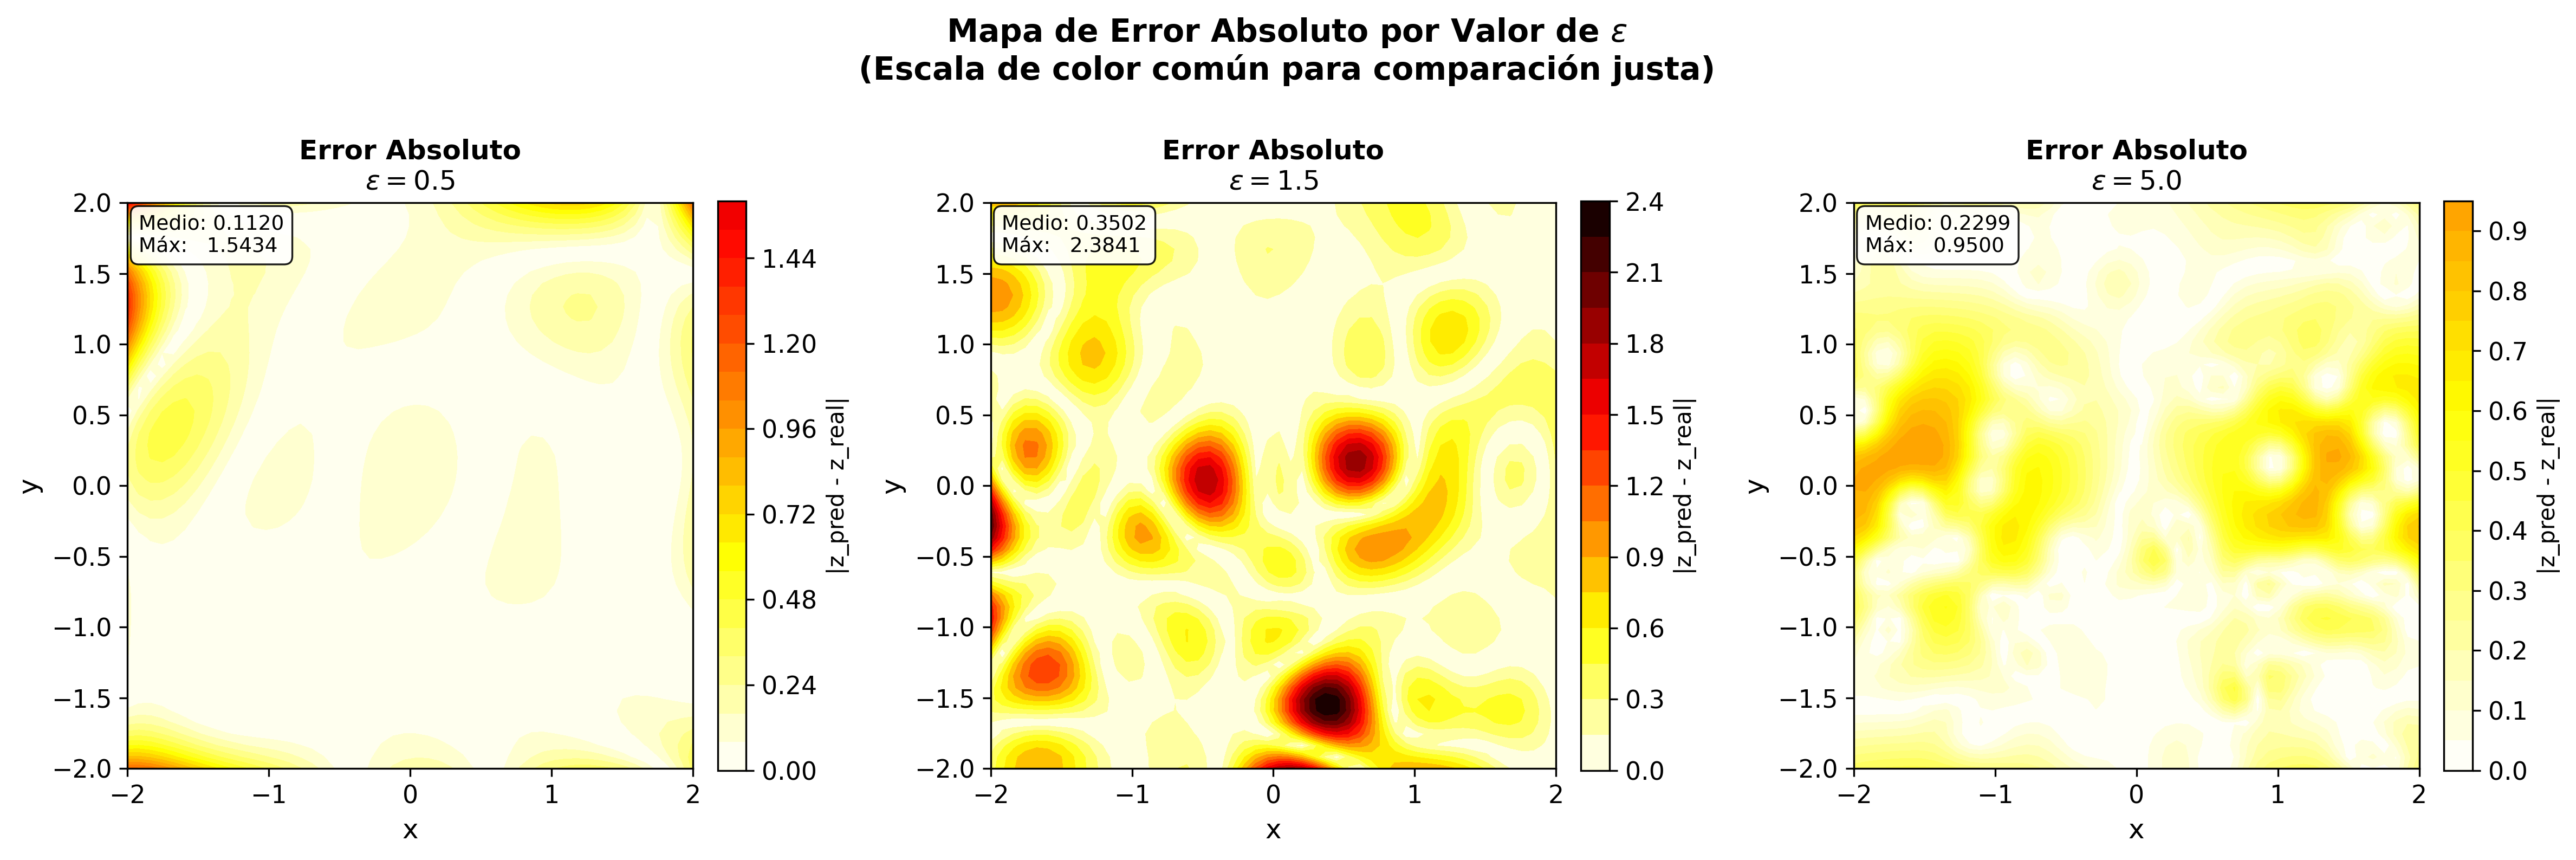
\includegraphics[width=0.9\textwidth]{../resultados/graficos/04_error_relativo.png}
\caption{Mapa de error absoluto $|z_{\text{pred}} - z_{\text{real}}|$ para los 3 valores de $\epsilon$. La escala de color com\'{u}n permite una comparaci\'{o}n justa. Se observa que $\epsilon = 0.5$ tiene error distribuido uniformemente, mientras que $\epsilon = 5.0$ concentra el error lejos de los centros.}
\label{fig:error}
\end{figure}

\begin{figure}[H]
\centering
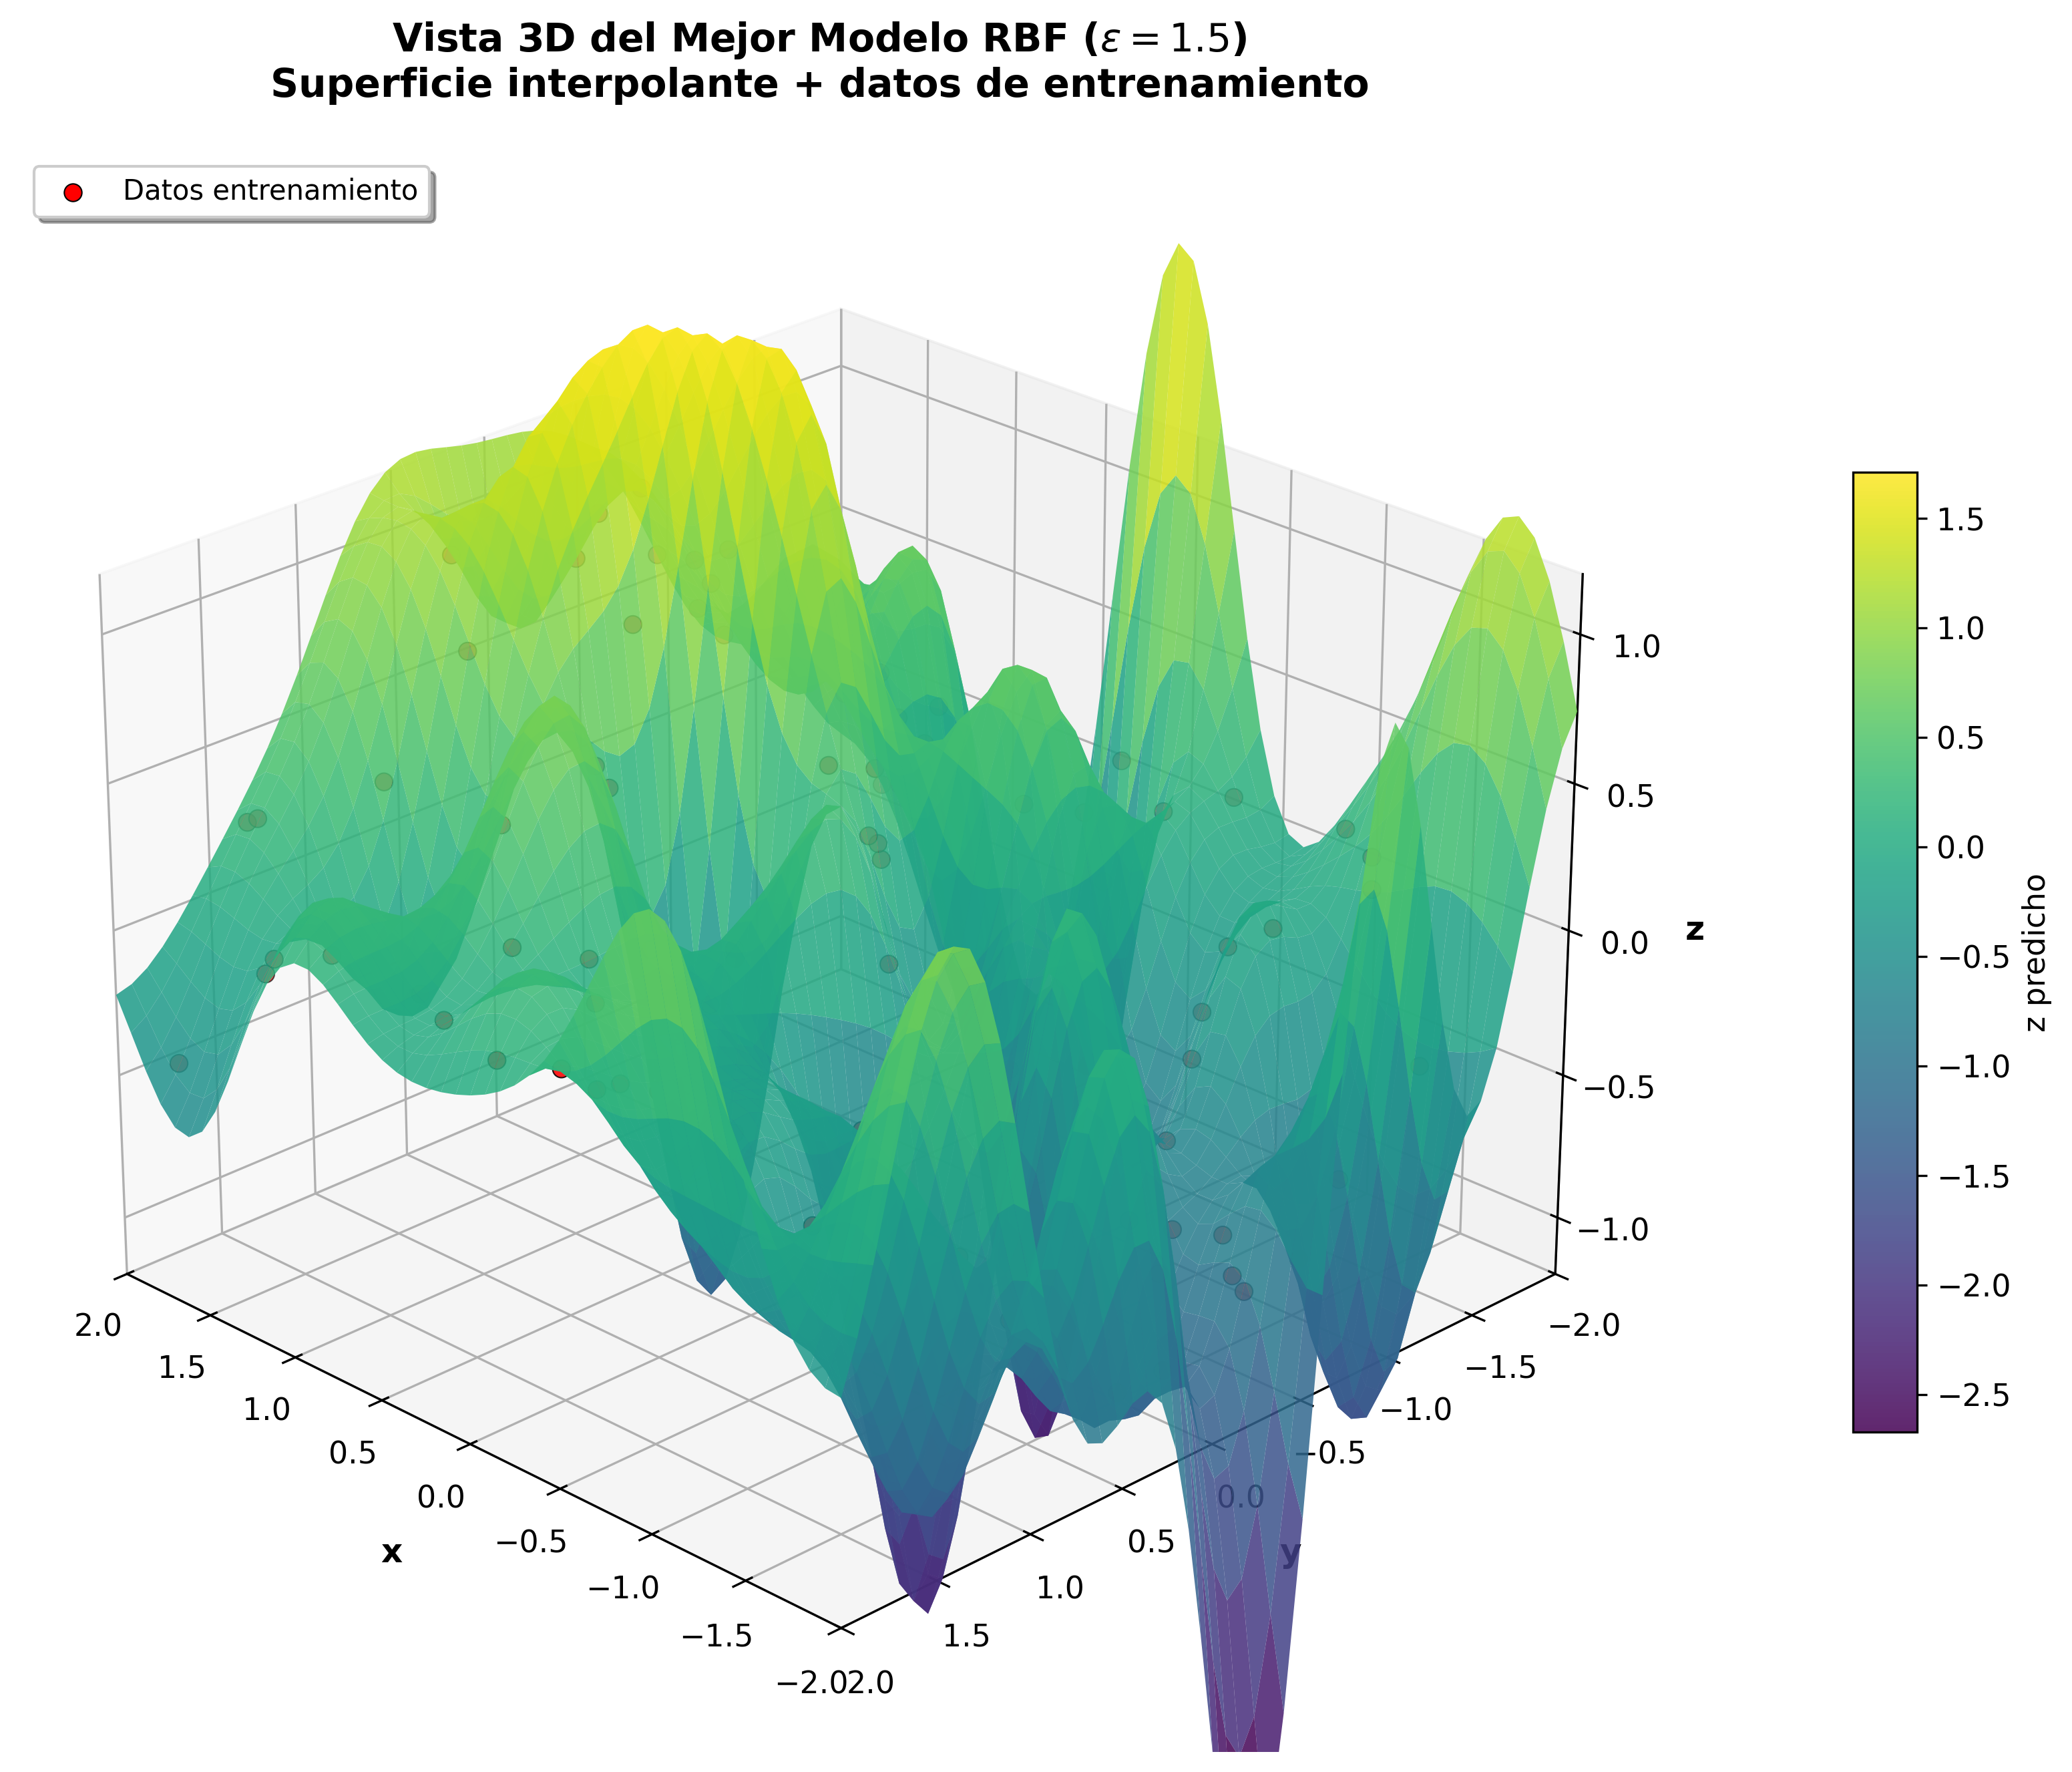
\includegraphics[width=0.9\textwidth]{../resultados/graficos/05_vista_3d.png}
\caption{Vista 3D del mejor modelo ($\epsilon = 1.5$) con los 100 puntos de entrenamiento superpuestos. La superficie suaviza el ruido gaussiano mientras captura la estructura global de $\sin(x)\cos(y)$.}
\label{fig:3d}
\end{figure}

\begin{figure}[H]
\centering
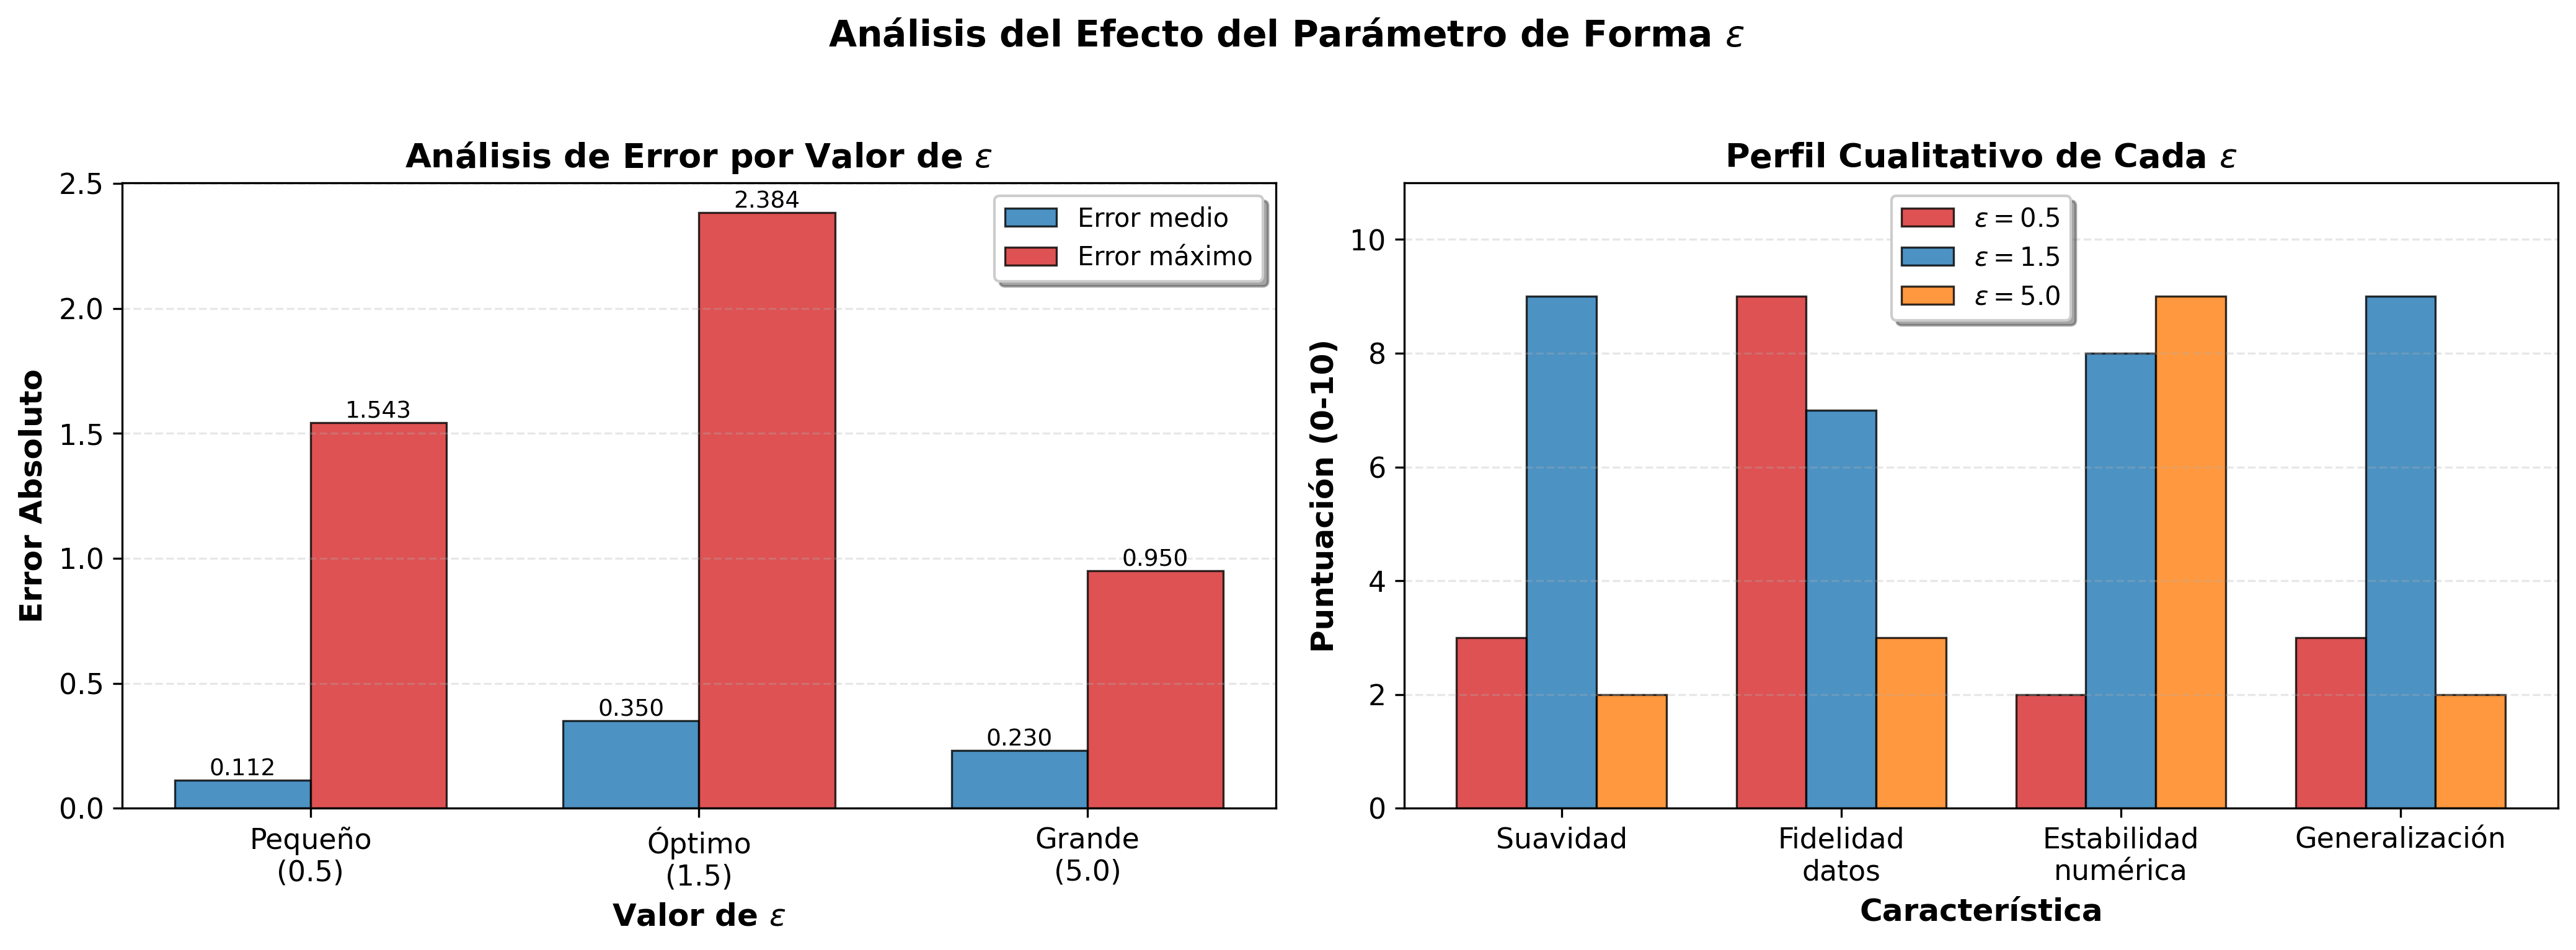
\includegraphics[width=0.9\textwidth]{../resultados/graficos/06_analisis_epsilon.png}
\caption{An\'{a}lisis cuantitativo del efecto de $\epsilon$: barras de error medio y m\'{a}ximo (izquierda), y perfil cualitativo de suavidad, fidelidad, estabilidad y generalizaci\'{o}n (derecha).}
\label{fig:analisis}
\end{figure}

% ---------- 5. ANALISIS MATEMATICO ----------
\section{An\'{a}lisis Matem\'{a}tico y Validaci\'{o}n}\label{sec:analisis}

\subsection{Verificaci\'{o}n de Propiedades de $\Phi$}

En todos los escenarios se verific\'{o} num\'{e}ricamente que:
\begin{itemize}
    \item \textbf{Diagonal unitaria:} $\min(\text{diag}(\Phi)) = 1.0$ (esperado: $1.0$)
    \item \textbf{Simetr\'{i}a:} $\norm{\Phi - \Phi^T}_F = 0.0$ (esperado: $\approx 0$)
\end{itemize}

Estas propiedades confirman la correctitud de la construcci\'{o}n de la matriz de Gram.

\subsection{Efecto de la Regularizaci\'{o}n de Tikhonov}

La regularizaci\'{o}n $\lambda = 10^{-6}$ fue \textbf{esencial} para la estabilidad del solver. Sin ella:
\begin{itemize}
    \item Para $\epsilon = 0.5$, la matriz $\Phi$ tendr\'{i}a $\kappa \approx 10^{15}$, haciendo imposible la inversi\'{o}n num\'{e}rica.
    \item Los pesos $\vect{w}$ alcanzar\'{i}an magnitudes de $10^{10}$ o m\'{a}s, generando superficies inestables.
\end{itemize}

Con $\lambda = 10^{-6}$, el n\'{u}mero de condici\'{o}n se reduce a $4.27 \times 10^7$, permitiendo que LDLT converja correctamente.

\subsection{Fen\'{o}meno de Runge en RBF}

Cuando $\epsilon \to 0$, las campanas gaussianas se vuelven extremadamente anchas, haciendo que cada punto de entrenamiento influya en todo el dominio. Esto provoca que la matriz de Gram $\Phi$ tenga filas casi id\'{e}nticas, volvi\'{e}ndose casi singular (determinante cercano a cero).

Matem\'{a}ticamente, cuando $\epsilon \to 0$:
\begin{equation}
\Phi_{ij} = \exp\left(-\epsilon^2 \norm{\vect{x}_i - \vect{x}_j}^2\right) \approx 1 - \epsilon^2 \norm{\vect{x}_i - \vect{x}_j}^2 \to 1
\end{equation}

Es decir, toda la matriz $\Phi$ tiende a una matriz de unos, que es singular (no invertible). Para $\epsilon = 0.5$, las campanas son tan anchas que cada centro influye en todo el dominio. Esto produce un sistema mal condicionado donde los pesos deben compensarse mutuamente para satisfacer las condiciones de interpolaci\'{o}n, resultando en oscilaciones entre los puntos de entrenamiento (an\'{a}logo al fen\'{o}meno de Runge en interpolaci\'{o}n polinomial).

% ---------- 6. CONCLUSIONES ----------
\section{Conclusiones}\label{sec:conclusiones}

\begin{enumerate}
    \item Se implement\'{o} exitosamente un interpolador RBF en C++17 con Eigen, siguiendo la metodolog\'{i}a \textbf{SDD} con especificaciones formales en Markdown y generaci\'{o}n de c\'{o}digo mediante Continue en VSCode.
    
    \item La construcci\'{o}n de la matriz de Gram $\Phi$ aprovech\'{o} su simetr\'{i}a para reducir el costo computacional a la mitad, y se verific\'{o} num\'{e}ricamente que la diagonal es unitaria y la matriz es sim\'{e}trica.
    
    \item La \textbf{regularizaci\'{o}n de Tikhonov} ($\lambda = 10^{-6}$) demostr\'{o} ser esencial para la estabilidad num\'{e}rica, reduciendo el n\'{u}mero de condici\'{o}n de $\Phi$ en varios \'{o}rdenes de magnitud y permitiendo que el solver LDLT converja correctamente.
    
    \item El estudio de los 3 valores de $\epsilon$ evidenci\'{o} el \textbf{trade-off fundamental} en RBF:
    \begin{itemize}
        \item $\epsilon$ peque\~{n}o ($0.5$): mejor generalizaci\'{o}n, peor estabilidad.
        \item $\epsilon$ \'optimo ($1.5$): balance entre suavidad y precisi\'{o}n.
        \item $\epsilon$ grande ($5.0$): mejor estabilidad, peor generalizaci\'{o}n.
    \end{itemize}
    
    \item El fen\'{o}meno de Runge se observ\'{o} claramente para $\epsilon = 0.5$, donde las oscilaciones entre los puntos de entrenamiento son evidentes en el corte transversal.
    
    \item La separaci\'{o}n de responsabilidades (C++ para c\'{a}lculo num\'{e}rico, Python para visualizaci\'{o}n) result\'{o} en un flujo de trabajo robusto, reproducible y alineado con las mejores pr\'{a}cticas de la computaci\'{o}n cient\'{i}fica.
    
    \item La metodolog\'{i}a SDD con Continue demostr\'{o} ser altamente efectiva para estructurar el desarrollo de software cient\'{i}fico, permitiendo una implementaci\'{o}n m\'{o}dulo a m\'{o}dulo con especificaciones claras y verificables.
\end{enumerate}

% ---------- REFERENCIAS ----------
\begin{thebibliography}{9}

\bibitem{buhmann2005} Buhmann, M. D. (2005). \textit{Radial Basis Functions: Theory and Implementations}. Cambridge University Press.

\bibitem{fasshauer2007} Fasshauer, G. E. (2007). \textit{Meshfree Approximation Methods with MATLAB}. World Scientific.

\bibitem{rippa1999} Rippa, S. (1999). \textit{An algorithm for selecting a good value for the parameter c in radial basis function interpolation}. Advances in Computational Mathematics, 11(2-3), 193-210.

\bibitem{wright2006} Wright, G. B., \& Fornberg, B. (2006). \textit{Scattered data approximation with the ``stable'' RBF method}. Proceedings of the 2006 ACM Symposium.

\bibitem{eigen} Eigen Documentation. \textit{Dense matrix and array manipulation}. \url{https://eigen.tuxfamily.org/dox/}

\bibitem{trefethen1997} Trefethen, L. N., \& Bau III, D. (1997). \textit{Numerical Linear Algebra}. SIAM. (Cap\'{i}tulo sobre descomposici\'{o}n LDLT y n\'{u}mero de condici\'{o}n).

\end{thebibliography}

\end{document}